 

%\part{Muestreo}
%\frame{\titlepage}
%\section[Índice]{Distribuciones en las muestras y descripción de datos.}
\chapter{Muestreo.}
%\frame{\tableofcontents}

%\renewcommand{\thepart}{2}
%\part{Muestreo.}

\section{Muestreo Estadístico}
  \begin{frame}
\begin{itemize}
   \item En esta tema sentaremos las bases del muestreo estadístico.
   \item Estudiaremos las distribuciones de algunos estadísticos muestrales; como la media aritmética, la proporción y la varianza.
  \end{itemize}
\end{frame}

\section{Conceptos básicos}
\begin{frame}
\frametitle{Conceptos básicos}
\begin{itemize}
 \item Ya hemos estudiado algunos de los conceptos básicos sobre muestras
\item Ahora los repasaremos y ampliaremos.
\item Recordemos:
  \begin{itemize}
  \item \textbf{Población}: Conjunto de individuos con una característica observable
  común.
  \item \textbf{Muestra}: Subconjunto de la población del que se espera que la
  represente.
\end{itemize}
\end{itemize}
\end{frame}

\begin{frame}
\frametitle{Análisis exploratorio, análisis confirmatorio}


\begin{itemize}
 \item Si tenemos información o datos que estudian un determinado fenómeno, podemos realizar un \textbf{análisis exploratorio}. Es decir, 
analizaremos, resumiremos e intentaremos interpretar los datos.
\item Otra situación puede ser contrastar o testear una hipótesis sobre el comportamiento de unos determinados datos.
\item Para confirmar dicha hipótesis, diseñaremos un estudio estadístico. A partir de dicho estudio, confirmaremos o refutaremos la hipótesis.
\item Dicho estudio estadístico consistirá en el diseño de un experimento que incluye una recogida de datos.
\item Dicho estudio estadístico se denomina \textbf{análisis de datos confirmatorio}, con el que queremos reforzar y aportar evidencias sobre 
la veracidad de nuestra hipótesis.
\end{itemize}
\end{frame}


\begin{frame}
\frametitle{La estadística inferencial}
\begin{itemize}
\item En los estudios de tipo \textbf{exploratorio}, la estadística descriptiva es  una de las herramientas principales.
\item  En los estudios de tipo \textbf{confirmatorio} lo es la \textbf{estadística inferencial}
\item  El objetivo de la \textbf{estadística inferencial} es obtener
  información sobre el conjunto de la población a partir de un
  subconjunto representativo de ella llamado muestra.
\item \textbf{Inferir información} de una muestra es contestar
  preguntas sobre el total de la población a partir del estudio de una muestra
  representativa de la misma.
\end{itemize}
\end{frame}

\begin{frame}
 
  \subsubsection{Pasos en un estudio inferencial}
\frametitle{Pasos en un estudio inferencial}

Los siguientes son unos pasos habituales en un estudio inferencial:
  
\begin{itemize}
      \item ¿Qué información se necesita?
      \item ¿Cuál es la información relevante? ¿Se dispone de acceso
      a todos los individuos de la población?
      \item ¿Cómo seleccionamos los individuos de la muestra?
      \item ¿Qué método emplearemos para obtener la información de
      los individuos de la muestra?
      \item ¿Qué herramientas  utilizaremos para hacer inferencias?
      \item  ¿Qué conclusiones podemos obtener?
      \item   Si las conclusiones son fiables y suficientes,
      redactar informe; en caso contrario, se vuelve a empezar.
  \end{itemize}
\end{frame}

\begin{frame}
\subsection{Diseño de experimentos, técnicas de muestreo}
\begin{itemize}
\item El objetivo de las técnicas de muestreo es encontrar métodos para seleccionar muestras representativas de la población.
\item Las técnicas básicas son: el muestreo aleatorio simple, el muestreo aleatorio estratificado, el muestreo sistemático y el muestreo polietápico. 
Cada una de estas técnicas proporciona una muestra representativa de la población.
\item Describiremos de forma breve estas técnicas.
\end{itemize}
\end{frame}

\begin{frame}
\frametitle{Muestreo aleatorio probabilístico}
\begin{itemize}
\item El muestreo aleatorio consiste en seleccionar muestra de la población con igual probabilidad.
\item Lo que equivale a que cualquier conjunto de individuos tiene la misma probabilidad de ser seleccionado. 
\item Pensemos en una urna con $100$ bolas de colores. Hay dos maneras de obtener una muestra de $10$ bolas.
\item Una podría ser sacar una bola de la urna, observar su color y devolverla a la urna.
\item Es decir vamos obteniendo individuos y los volvemos a poner en la urna. 
\item Este tipo de muestreo recibe el nombre de \textbf{muestreo con reposición} o \textbf{muestreo aleatorio simple}.
\end{itemize}
\end{frame}

\begin{frame}
\frametitle{Muestreo aleatorio probabilístico}
\begin{itemize}
\item Otra forma sería repetir la experiencia anterior pero no devolver las bolas a la urna.
\item  En este caso también sucede que cualquier selección de los $10$ individuos es equiprobable. 
En este caso se habla de \textbf{muestreo aleatorio sin reposición}.
\item Cuando el tamaño de la población sea muy grande en relación a la muestra y por lo tanto la probabilidad de que dos individuos se repitan 
sea muy pequeña, el muestreo aleatorio con reemplazo  y el muestreo aleatorio sin reemplazo serán aproximadamente equivalentes.
\item De todas maneras, si el tamaño de la población es pequeño, se suelen aplicar estadísticos corregidos por el efecto del
tamaño de la población.
\end{itemize}
\end{frame}

\begin{frame}
\frametitle{Muestreo Aleatorio Estratificado}
\begin{itemize}
\item Se utiliza en  el caso en que la población  esté dividida en grupos o estratos y que éstos sean de interés para la variable de estudio.
\item Se toman muestras donde cada grupo esté representado en función de su tamaño. 
\item Por ejemplo los estratos podrían ser los grupos de edad; o en las Islas Baleares, los estratos podrían ser las islas en proporción a 
su número de habitantes; o en una provincia, los estratos podrían ser los municipios también en función de su número de
habitantes,
o los estratos se podrían diseñar según el nivel educativo de sus habitantes, etc.
\item En estos casos Se determina el tamaño de la muestra en cada estrato y luego se toma una muestra aleatoria simple en ese bloque.
\end{itemize}
\end{frame}

\begin{frame}  
\frametitle{Muestreo por conglomerados}
\begin{itemize}
\item El proceso de obtener una muestra aleatoria en algunos casos es caro.
\item Por ejemplo, si el estudio se realiza sobre conjuntos de personas, tener una lista completa de dichas personas puede ser muy costoso.
 Imaginemos que queremos saber los hábitos de alimentación que tienen los estudiantes de Primaria de Baleares. 
\item Para ello, previo permiso de la autoridad responsable, queremos seleccionar una muestra representativa de los escolares de Baleares. 
\item En vez de hallar una muestra representativa de todos los estudiantes de Primaria, elegimos al azar primeramente un conjunto de colegios a los que 
llamamos conglomerados.
\item Seguidamente, dentro de cada colegio (conglomerado) elegimos al azar un conjunto de estudiantes. Pensemos que es mucho más
sencillo poseer
una lista completa de estudiantes de una serie de colegios que poseer una lista completa de todos los estudiantes. 
\end{itemize}
\end{frame}

\begin{frame}
\begin{itemize}
\item Cuando no se da algún tipo de aleatoriedad en la selección de la muestra se habla de  \textbf{muestreo no probabilístico}.
\item Suele ser frecuente este tipo de muestreo. En muchos casos,  nos tenemos que conformar con la información disponible o  
la obtenida voluntariamente.
\item Existen \textbf{otros tipos} de muestreo que suelen ser combinaciones de las técnicas anteriores y otro tipos de técnicas.
\item En cualquier caso, lo importante es que  el estudio estadístico que se realiza ``a posteriori'' es diferente según el muestreo realizado.
\end{itemize}
\end{frame}

\begin{frame}
\frametitle{Diferentes tipos de muestreo, diferentes estadísticos}
\begin{itemize}
\item Una vez realizado el muestreo y obtenidos los datos (``raw data''), hemos de explicar cómo obtener estadísticos a partir de dichos datos como 
pueden ser proporciones, medias, varianzas, etc.
\item La forma de obtener dichos estadísticos se realiza mediante los llamados estimadores. O sea, un estimador es simplemente una fórmula a aplicar 
a los datos del muestreo para obtener el valor de dicho estadístico.
\item El ejemplo más conocido es la media aritmética: sean $x_1,\ldots,x_n$ los datos del muestreo. El estimador que nos da la media aritmética es:
\[
\overline{x}=\frac{x_1+\cdots +x_n}{n}.
\]
\item En este curso estudiaremos técnicas de estimación para el caso de  muestreo aleatorio simple.
\end{itemize}
\end{frame}

\subsubsection{Muestreo aleatorio simple}

\begin{frame}
\frametitle{Muestreo aleatorio simple}
\begin{itemize}
\item Estudiemos un poco más en detalle el caso del muestreo aleatorio simple con o sin reposición.
\item La idea es que queremos seleccionar una muestra de tamaño $n$ (es decir formada por $n$ individuos) 
de una población de tamaño $N$.
\item Obtendremos una muestra aleatoria simple (m.a.s.) cuando todas las muestras posibles de $n$ individuos tengan la misma probabilidad de ser elegidas.
\item El tener una m.a.s de una población junto con un tamaño muestral adecuado nos asegurará la suficiente representatividad  de la muestra.
\end{itemize}
\end{frame}

\begin{frame}
\frametitle{Observaciones sobre el muestreo aleatorio simple}
Hagamos algunas observaciones:
\begin{itemize}
\item El proceso mismo del muestreo aleatorio simple es complejo.
\item Una forma sencilla es numerar, si es posible a todos los individuos de la población y sortearlos eligiendo números como si se tratase de una lotería.
\item Por ejemplo con una tabla de números aleatorios o con algún generador de números aleatorios.
\footnote{En realidad los números aleatorios generados por diversos tipos de algoritmos  son pseudoaleatorios; son números que
superan 
determinados test de aleatoriedad} Tanto los paquetes estadísticos como \texttt{R} o las hojas de cálculo como \texttt{Open
Office} 
tienen generadores de números aleatorios.
% \begin{enumerate}[a)]
% \item Población mundial de seres humanos.
% \item Población de llamadas a una centralita telefónica.
% \item Población de votantes en las próximas elecciones locales y autonómicas.
% \end{enumerate}
% \item En algunos de estos casos será luego impracticable localizar alos individuos seleccionados y convencerlos de que respondan, quizás muchos no querrán.
\end{itemize}
\end{frame}

\subsubsection{Estadísticos y distribuciones muestrales} 

\begin{frame}
\frametitle{Inferencias}
\begin{itemize}
\item Una vez definido nuestro valor de interés y el estimador que lo estima o calcula, necesitamos estudiar dicho estimador.
\item Por ejemplo, supongamos que tenemos una muestra aleatoria simple de una población y deseamos obtener información sobre la media o 
la varianza poblacionales. 
\item Para obtener dicha información sobre la media o la varianza, necesitamos definir los estimadores para calcular dichos valores a partir de los
valores de la muestra. Dichos estimadores se denominan \textbf{estadísticos}.
\item Un \textbf{estadístico} es una función que depende de la
muestra.
\item  Pensemos por ejemplo en la media aritmética, proporción muestral, etc.
\end{itemize}
\end{frame}

\subsubsection{Distribución muestral de un estadístico}

\begin{frame}
\frametitle{Distribución muestral de un estadístico}
\begin{itemize}
\item Desde el punto de vista teórico, una m.a.s. es un conjunto de $n$ variables aleatorias independientes e idénticamente distribuidas según 
la distribución de la variable aleatoria~$X$, que representa la variable de estudio. Escrito de forma
matemática: $X_1,\ldots, X_n$.
\item La muestra aleatoria serían unos determinados valores que cogen dichas variables aleatorias: $x_1,\ldots,x_n$.
\item Por tanto, al ser los estadísticos funciones de la muestra, serán funciones de las variables $X_1,\ldots,X_n$: $T=f(X_1,\ldots,X_n)$, donde $T$ 
representa el estadístico y $f$ la función a considerar.
\item En el caso de la media aritmética, tenemos que $f(X_1,\ldots,X_n)=\frac{X_1+\cdots +X_n}{n}$.
\item Un estadístico $T$ será por tanto una variable aleatoria, desde el punto de vista teórico.
\item La \textbf{distribución muestral o distribución en el muestreo} de un estadístico $T$ será la
distribución de probabilidad de la variable aleatoria~$T$.
\end{itemize}
\end{frame}

\begin{frame}
\frametitle{Ejemplo}
\begin{itemize}
\item Supongamos que queremos estimar cuál es número medio de pruebas de embarazo defectuosas, de una
 determinada marca, que hay en cada caja de 10 unidades cada una.
\item  Para ello tomamos una muestra aleatoria simple de cuatro cajas 
$X_{1}$, $X_{2}$,$X_{3}$, $X_{4}$.
\item Se comprueba si son correctas o no y  obtenemos  los siguientes resultados:
\begin{center}
      \begin{tabular}{lcccl}
     primera caja &: & $x_1$ &  1 &defectuosa\\
     segunda caja &: & $x_2$ & 2 &defectuosas\\
     tercera caja &: & $x_3$ & 0 &defectuosas\\
     cuarta  caja &: & $x_4$ &1 &defectuosas
     \end{tabular}
\end{center}
\end{itemize}
\end{frame}

\begin{frame}
     Definimos el estadístico media aritmética de  pruebas defectuosas como:

     $$\overline{X}=f(X_{1}, X_{2}, X_{3},
     X_{4})=\frac{X_{1}+X_{2}+X_{3}+X_{4}}{4}$$

     En este caso $\overline{X}=1$.
\end{frame}


\begin{frame}
   Supongamos que tomamos repetidas muestras de tamaño 4, los
     resultados son:
\begin{center}
     \begin{tabular}{c|c|c|c|c|c|c|c|c|c}
      M. & M. & M. & M. & M. & M. & M. & M. & M. & M.\\
1 & 2 & 3 & 4 & 5 & 6 & 7 & 8 & 9 & 10 \\ \hline 0&1&3&0&0&1&0&0&0&1\\
1&1&1&0&1&1&1&0&0&2\\ 0&1&2&1&0&0&1&2&0&1\\ 1&1&2&2&1&3&0&0&1&1
\end{tabular}
\end{center}

\begin{center}
     \begin{tabular}{c|c|c|c|c|c|c|c|c|c}
     M. & M. & M. & M. & M. & M. & M. & M. & M. & M.\\
11 & 12 & 13 & 14 & 15 & 16 & 17 & 18 &  19 & 20 \\
 \hline
0&0&1&2&0&2&1&2&1&1\\ 1&0&1&0&1&1&2&0&0&1\\ 1&0&2&0&1&1&0&1&1&0\\ 3&3&1&0&0&2&1&0&1&1
\end{tabular}
\end{center}

\end{frame}
\begin{frame}
Las medias aritméticas de cada muestra son:
\begin{center}
\begin{tabular}{ccccc}
 0.50&1.00&2.00&0.75&0.50\\
 1.25&0.50&0.50&0.25&1.25\\
 1.25&0.75&1.25&0.50&0.50\\
 1.50&1.00&0.75&0.75&0.75
  \end{tabular}
  \end{center}
  %\end{example}
\end{frame}

\begin{frame}
  Entonces:
  $$P_{\overline{X}}(0.25))=P(\overline{X}=0.25)=\frac{1}{20}=0.05$$
  $$P_{\overline{X}}(0.50))=P(\overline{X}=0.50)=\frac{6}{20}=0.30$$
  $$P_{\overline{X}}(0.75))=P(\overline{X}=0.75)=\frac{5}{20}=0.25$$
  $$P_{\overline{X}}(1))=P(\overline{X}=1)=\frac{2}{2}=0.10$$
  $$P_{\overline{X}}(1.25))=P(\overline{X}=1.25)=\frac{4}{20}=0.20$$
  $$P_{\overline{X}}(1.50))=P(\overline{X}=1.5)=\frac{1}{20}=0.05$$
  $$P_{\overline{X}}(2))=P(\overline{X}=2)=\frac{1}{20}=0.05$$

   Esta sería una aproximación a la distribución muestral del
   estadístico $\overline{X}$ a partir de los datos de varias
   muestras.

\end{frame}

\subsection{Distribución  de la media muestral}

\begin{frame} 
\frametitle{Distribución de la media muestral}
\begin{itemize}
\item La distribución del estadístico puede seguir un modelo preestablecido si se cumplen varias condiciones.
\item Por ejemplo, supongamos que hemos tomado una muestra aleatoria simple de $n$ observaciones
 de una v.a. $X$ en una población de media $\mu_{X}$ y desviación típica $\sigma_{X}$.
\item Representemos por $X_{1}, X_{2},\ldots,X_{n}$  
 $n$ observaciones independientes que forman
 una muestra aleatoria simple de ésta población.
\item  Cada una de las observaciones de la población son así mismo variables aleatorias con la misma distribución, esperanza y varianza  
que la población.
\end{itemize}
\end{frame}

\begin{frame}
\frametitle{Estadístico media muestral}
\begin{itemize}
\item Llamaremos \textbf{media aritmética o media muestral}  de la muestra
 $X_{1},\ldots,X_{n}$ al estadístico o variable aleatoria siguiente:
 $$\overline{X}=\frac{\sum_{i=1}^n X_{i}}{n}$$.
\item Bajo estas condiciones se cumple que:

\begin{enumerate}[a)]
\item $E(\overline{X})=\mu_{X}$.
\item  Es decir, el valor esperando de la media aritmética de la muestra es la media
 poblacional. 
\item Por lo tanto  el estadístico media muestral \textbf{estima} la media poblacional.
\item  Dicho  de  otra forma, la esperanza de la distribución muestral de la media aritmética es la media poblacional.
\end{enumerate}
\end{itemize}
\end{frame}

\begin{frame}
\begin{itemize}
\item  Que el valor esperado sea $\mu_{X}$, no quiere decir que $\overline{X}$ sea exactamente~$\mu_{X}$. 
\item  Estudiemos la varianza de $\overline{X}$. Si  $X_{1},\ldots,X_{n}$ son independientes se cumple que:
\begin {enumerate}[a)]
\item $Var(\overline{X})=\frac{1}{n} \sigma_{X}^2$.
\item Luego  si $n$ es suficientemente grande (o cuando $n\to\infty$) la varianza tenderá a estar muy próxima a cero.
\end{enumerate}
\end{itemize}
\end{frame}

\begin{frame}
\frametitle{Ejemplo}
\begin{itemize}
\item 
Veamos con un ejemplo que la independencia entre $X_{1},\ldots,X_{n}$ no siempre está asegurada.
\item  Por ejemplo  en el caso en el  que queramos averiguar cuántos votos
 afirmativos hay en una urna con $10$ votos.
\item  Tenemos dos opciones para realizar la muestra aleatoria simple:
 \begin{enumerate}[a)]
 \item Tomar un voto al azar, anotar su resultado y devolverlo a la urna y
 repetir el proceso $3$ veces más. En este caso es un muestreo con reemplazamiento.
 \item Tomar sucesivamente $4$ votos de la urna sin reemplazarlos.
 En este caso es un muestreo  sin reemplazamiento.
 \end{enumerate}
\end{itemize}
\end{frame}

\begin{frame}
\begin{itemize}
\item  En ambos casos la muestra obtenida es una muestra aleatoria  pues todos los
 subconjuntos de individuos tienen igual probabilidad de ser elegidos.
\item  Pero en el primer caso tenemos independencia entre cada una de las
 observaciones mientras que en el segundo esto no es así.
\end{itemize}
\end{frame}
\begin{frame}
\begin{itemize}
\item  En la práctica se elige casi siempre el muestreo consistente en
 observar $n$ individuos distintos.
\item  Si además, $n$ es pequeño con respecto al tamaño de la población $N$,
 podemos suponer que las variables son prácticamente independientes.
\item En caso contrario, tenemos que corregir la varianza  de $\overline{X}$ multiplicándola por lo que se
 denomina \textbf{factor de población finita} y tendremos que

 $$\sigma_{\overline{X}}^2=Var(\overline{X})=\frac{1}{n} \sigma_{X}^2 \frac{(N-n)}{(N-1)}$$
\end{itemize}
\end{frame}

\begin{frame}
\frametitle{Tipificación de la media muestral. Teorema del Límite Central}
\begin{itemize}
\item Frecuentemente utilizaremos la \textbf{expresión tipificada de la media muestral}:
 $$Z=\frac{\overline{X}-\mu_{\overline{X}}}{\sigma_{\overline{X}}}
 =\frac{\overline{X}-\mu_{X}}{\frac{\sigma_{X}}{\sqrt{n}}}$$
\item  Además para  tamaños muestrales grandes se cumple  el  importantísimo \textbf{Teorema del Límite Central} que afirma que  la
 distribución de $Z$ es aproximadamente una normal estándar.
\item  Este resultado es cierto \textbf{sea cual sea la distribución de la variable muestreada~$X$.}
\item Deducimos por tanto, usando las propiedades de la distribución normal, que la distribución de
  $\overline{X}$ será aproximadamente normal si $n$ es suficientemente grande.
\end{itemize}
\end{frame}

\begin{frame}
\frametitle{Propiedades de la media muestral}
Sea $X$ la variable aleatoria de interés que queremos observar en  una cierta población. Supongamos que 
 la esperanza poblacional es  $E(X)=\mu_{X}$ y su  varianza $Var(X)=\sigma_{X}^2$. Sea
$X_{1},\ldots, X_{n}$ una muestra aleatoria simple de dicha población:

Entonces se cumplen las propiedades siguientes:

\begin{itemize}
\item $\mu_{\overline{X}}=E(\overline{X})=\mu_{X}$; el valor esperado de la media es la media poblacional.
\item La varianza y la desviación típica de $\overline{X}$ se pueden obtener con las siguientes fórmulas $\sigma_{\overline{X}}^2=\frac{1}{n}\sigma_{X}^2$, $\overline{X}$ es $\sigma_{\overline{X}}=
 \frac{\sigma_{X}}{\sqrt{n}}$
 que también recibe el nombre de \textbf{error estándar} de $\overline{X}$.
\item Para poblaciones finitas de tamaño $N$ si $n$  es pequeño respecto de $N$
hemos de  aplicar el factor de corrección de población finita en
  el cálculo de la varianza y del error estándar de $\overline{X}$:

 $$\sigma_{\overline{X}}^2=\frac{1}{n}\sigma_{X}^2\frac{(N-n)}{(N-1)},\quad
\sigma_{\overline{X}}=\frac{\sigma_{X}}{\sqrt{n}}\sqrt{\frac{(N-n)}{(N-1)}}$$
 
\end{itemize}
\end{frame}

\begin{frame}
%\frametitle{}
\begin{itemize}
\item  Si la distribución de la población ($X$) es normal, entonces
 la variable aleatoria:
 $$Z=\frac{\overline{X}-\mu_{X}}{\frac{\sigma_{X}}{\sqrt{n}}}$$

 es una normal estándar. O lo que es lo mismo $\overline{X}$ es una
 normal con media $\mu_{X}$ y  desviación típica
 $\sigma_{\overline{X}}$
 \item \textbf{Teorema del Límite Central:} Si la distribución de la población no es normal pero el tamaño
 muestral es suficientemente grande entonces por el T.L.C.
 la distribución de $Z$ también se aproxima a una normal estándar y
 por lo tanto $\overline{X}$ se aproxima a una
 normal con media $\mu_{X}$ y  desviación típica
 $\sigma_{\overline{X}}$
\end{itemize}
\end{frame}

\begin{frame}
\frametitle{Ejemplo}
    La altura media de  un determinado arbusto se sabe que tiene una media poblacional de $115$ centímetros y una desviación
    típica poblacional de $25$. Se toma una muestra aleatoria de $100$ arbustos de esta especie.
    \begin{enumerate}[a)]
        \item ¿Cuál es la probabilidad de que la media muestral de las
        de las alturas sea menor que $110$ cm.?
        \item ¿Cuál es la probabilidad de que la media muestral de las
        alturas esté entre $113$ cm. y $117$ cm.?
        \item ¿Cuál es la probabilidad de que la media muestral de las
        alturas esté entre $114$ cm.y $116$ cm.?
        \item Sin hacer cálculos, razonar en cuál de los siguientes rangos
        resulta más probable que se encuentre la media muestral de las
        alturas.
        \begin{center}
        \begin{tabular}{ll}
        113 cm.-&115 cm.\\
        114 cm.-&116 cm.\\
        115 cm.-&117 cm.\\
        116 cm.-&118 cm.
            \end{tabular}
            \end{center}
        \end{enumerate}
\end{frame}

\begin{frame}
\begin{itemize}
\item Supongamos que el número de individuos de la población de arbustos muy grande en relación al tamaño
muestral $n=100$.
\item  Sea $X$ es la v.a. altura de un arbusto en cm. 
\item Con los datos del enunciado tenemos que  $\mu_{X}=E(X)=115$ y $\sigma_{X}=25$.
\item  Sea 
$X_{1},\ldots,X_{100}$ la muestra aleatoria simple de alturas.
\item Tenemos que  $\mu_{\overline{X}}=\mu_{X}=115$ y
$\sigma_{\overline{X}}= \frac{\sigma_{X}}{\sqrt{n}}=\frac{25}{\sqrt{100}}=2.5$
\item Además, aplicando el T.L.C.,  se tiene que $Z=\frac{\overline{X}-\mu_{X}}{\frac{\sigma_{X}}{\sqrt{n}}}=
\frac{\overline{X}-115}{2.5}$.
 sigue aproximadamente una distribución normal estándar.
\end{itemize}
\end{frame}

\begin{frame}
     \textbf{Solución:}
\begin{enumerate}[a)]
 \item $P(\overline{X}\leq 110)= P(Z\leq \frac{110-115}{2.5})=$
 $P(Z\leq -2)=F_{Z}(-2)=1-F_{Z}(2)=1-0.9772=0.0228$.
\item $P(113\leq  \overline{X} \leq 117)= P(\frac{113-115}{2.5}\leq
  Z \leq \frac{117-115}{2.5})=$
  $F_{Z}(0.8)-F_{Z}(-0.8)=
  2 F_{Z}(0.8) -1= 2 (0.7881)-1=0.5762$.
\item $P(114\leq  \overline{X} \leq 116)= P(\frac{114-115}{2.5}\leq
  Z \leq \frac{116-115}{2.5})=$
  $F_{Z}(0.4)-F_{Z}(-0.4)=2 F_{Z}(0.8) -1= 2 (0.6554)-1=0.3108$.
\item La media aritmética de las alturas $\overline{X}$ sigue
  aproximadamente una distribución normal. Gráficamente el
  intervalo de mayor probabilidad será el que mayor área cubra bajo
  la curva normal (centrada en 115) y ese intervalo es
  114 cm.-116 cm.
\end{enumerate}
\end{frame}
    \subsection{Distribución de una proporción muestral}
\begin{frame}
    \frametitle{El estadístico proporción muestral}
\begin{itemize}
  \item  La proporción muestral de un evento en una población vendrá
    generalmente asociada a una variable binomial. Veamos por qué con un ejemplo.
\item 
    Si tomamos una muestra de tamaño $n$, determinar
    el porcentaje de personas que recicla las basuras. 
\item Sea $X_i$ la variable aleatoria que vale $0$ si la persona $i$-ésima no recicla y vale $1$ si la persona $i$-ésima recicla.
\item Tendremos que $S=\sum_{i}^{n}X_i$ nos dará el número total de personas que reciclan.
\item Llamamos $p$ a la probabilidad de que una persona elegida al azar recicle. Nuestro objetivo es estimar~$p$.
\item Suponiendo independencia y que el valor de $p$ no cambia para las personas, tendremos que la distribución de cada variable $X_i$ será 
de Bernoulli de parámetro~$p$ y, por tanto, la distribución de $S$ será binomial de 
parámetros~$n$ y~$p$.
\end{itemize}
\end{frame}
\begin{frame}
\begin{itemize}
\item  ¿Será realmente binomial? Notemos que en la
    muestra no preguntaremos dos veces al mismo individuo, (el muestreo es sin reposición).
    Luego las observaciones no son exactamente independientes,
    pero si el tamaño de la población es grande respecto a
    la muestra podemos considerarlas independientes, ya que la probabilidad de respuesta afirmativa no cambia.
    (es despreciable el cambio).
\end{itemize}
\end{frame}

\begin{frame}
\frametitle{Cálculo de la proporción muestral}
\begin{itemize}
\item Sea $S$ el número de éxitos en una muestra binomial de $n$
    observaciones, con probabilidad de éxito $p$.
\item  Entonces la
    proporción de éxitos en la muestra es:
    $$\hat{p}_{X}=\frac{S}{n},$$
  que recibe el nombre de  \textbf{proporción muestral}.
\end{itemize}
\end{frame}

    \subsubsection{Distribución en el muestreo de  $\mathbf{\hat{p}_{X}}$}

\begin{frame}
\frametitle{Propiedades de la proporción muestral}
    Sea   $\hat{p}_{X}$ la proporción de éxitos en una muestra
    aleatoria de $n$ observaciones. Entonces:

    \begin{itemize}
    \item  $E(\hat{p}_{X})=p$
    \item  La distribución muestral de $\hat{p}_{X}$  tiene
    varianza $\sigma_{\hat{p}_{X}}^2=\frac{p(1-p)}{n}$ y por lo tanto su desviación
    típica es
    $\sigma_{\hat{p}_{X} }=\sqrt{\frac{p(1-p)}{n}}$
    que recibe el nombre de \textbf{error estándar de la proporción
    muestral}.
    \item Si $n$ es pequeño en relación al tamaño de la población $N$
    tenemos que aplicar el factor de corrección de población finita
  y entonces el error estándar de  $\hat{p}_{X}$  es
    $$\sigma_{\hat{p}_{X} }=\sqrt{\frac{p(1-p)}{n}}
  \sqrt{\frac{N-n}{N-1}}.$$
\end{itemize}
\end{frame}

\begin{frame}
\frametitle{Distribución de la proporción muestral}
\begin{itemize}
  \item Si el tamaño muestral es grande (por ejemplo $n>30$ o mejor  $n>40$) entonces la variable
  $$Z=\frac{\hat{p}_{X}- p}{\sigma_{\hat{p}_{X}}},$$
  por el T.L.C., se distribuye aproximadamente como una normal estándar
  o lo que es lo mismo $\hat{p}_{X}$ se distribuye aproximadamente
  como una normal con esperanza $p_{X}$ y desviación típica
  $\sigma_{\hat{p}_{X}}$.
 
 \item \textbf{Observación} Notemos que si $n$ crece el error estándar
    disminuye y entonces $\hat{p}$ estará más cerca del valor real $p$.
\end{itemize}
\end{frame}

\begin{frame}
     \textbf{Ejemplo:}
 Se estima que el $20\%$ de los
    ciudadanos  separa el papel y el cartón cuando tira su basura. Cierto día
    utilizaron $n=180$ personas  uno de los puntos de recogida de basuras. Consideremos  estas personas como
    una muestra aleatoria de todos los ciudadanos.
        \begin{enumerate}[a)]
        \item ¿Cuál será la media de la proporción muestral de personas
        que reciclan papel?
        \item ¿Cuál es la varianza de la proporción muestral?
        \item ¿Cuál es el error estándar de la proporción muestral?
        \item ¿Cuál es la probabilidad de que la proporción muestral sea
        mayor que 0.15?
        \end{enumerate}
\end{frame}

\begin{frame}
   \textbf{Solución:}
    El tamaño de la muestra es pequeño en relación al
    número total de ciudadanos (si la ciudad es grande). Tenemos que $p=0.2$ (probabilidad
    de éxito en la venta).
\begin{itemize}
  \item $E(\hat{p}_{X})=p=0.2$

  \item $\sigma_{\hat{p}_{X}}^2= \frac{ p(1-p)}{n}=\frac{0.2
    (1-0.2)}{180}=0.0009$.
  \item $\sigma_{\hat{p}_{X}}=\sqrt{\frac{ p(1-p)}{n}}=\sqrt{0.0009}=0.03$.
    \item Como $n$  es grande entonces
    $Z=\frac{\hat{p}_{X}-p}{\sigma_{\hat{p}_{X}}}=\frac{\hat{p}_{X}-0.2}{0.03}$
 sigue aproximadamente una distribución normal estándar, entonces:

 $P(\hat{p}_{X}>0.15)=1-P(\hat{p}_{X}\leq 0.15)= 1-P(Z\leq
 \frac{0.15-0.2}{0.03})=1-F_{Z}( -1.67)=F_{Z}(1.67)=0.9525$.
\end{itemize}
\end{frame}

    \subsection{Distribución muestral de la varianza muestral}

\begin{frame}
\frametitle{La varianza muestral}

\begin{itemize}
\item Sea $X_{1},\ldots, X_{n}$ una muestra aleatoria simple de una población ($X$) con
$E(X)=\mu_{X}$ y $Var(X)=\sigma_{X}^2$. 
\item Llamaremos \textbf{varianza muestral} al estadístico:

$$\tilde{S}_{X}^2=\frac{\sum_{i=1}^n (X_{i}-\overline{X})^2}{n-1}.$$
\item 
$\tilde{S}_{X}=+\sqrt{\tilde{S}_{X}^2}$ recibe el nombre de desviación típica muestral.
\item 
Denotaremos por $S^2_{X}=\frac{(n-1)}{n}\tilde{S}^2_{X}$ y $S_X=+\sqrt{S_X^2}$.
\end{itemize}
\end{frame}

\begin{frame}
  \frametitle{Propiedades de la varianza muestral}
  \begin{itemize}
\item $S^2_X=\frac{\sum_{i=1}^n (X_{i}-\overline{X})^2}{n}=\left(\frac{\sum_{i=1}^n
X_{i}^2}{n}-\overline{X}^2\right)$
\item $E(S^2_X)=\frac{n-1}{n} \sigma^2_X$ (en el caso en que las variables $X_i$ sean normales)
\item $\tilde{S}_{X}^2=\frac{n}{n-1}\left(\frac{\sum_{i=1}^n
X_{i}^2}{n}-\overline{X}^2\right)$
\item $E(\tilde{S}_{X}^2)=\sigma_{X}^2$ (en el caso en que las variables $X_i$ sean normales)
\end{itemize}
\end{frame}

\subsubsection{Distribución en el muestreo de la varianza muestral}
    

\begin{frame}
\frametitle{Distribución de la varianza muestral}    
Con las notaciones anteriores tenemos que:

    \begin{itemize}
        \item $E(\tilde{S}_{X}^2)=\sigma_{X}^2$ (en el caso en que las variables $X_i$ sean normales)
      %%%%%%%%  \item Si la distribución de la población es normal entonces:
%%%%%%%%        $Var(\rilde{S}_{X}^2)=\frac{2\sigma_{X}^2}{n-1}$
        \item Si la distribución de la población es normal entonces
        la variable $\frac{(n-1)\tilde{S}_{X}^2}{\sigma_{X}^2}$ se distribuye
        según una ley conocida denominada $\chi_{n-1}^2$, que explicamos a continuación.
        \end{itemize}
\end{frame}

\begin{frame}
    \frametitle{La distribución $\chi^{2}_{n}$ (chi-cuadrado con $n$ g.l.)}
\begin{itemize}
\item Supongamos que  $X_{1},X_{2},\ldots, X_{n}$ son $n$  v.a. independientes y que $X_{i}\equiv N(0,1)$
\item  Entonces:
$$X=X_{1}^{2}+X_{2}^{2}+\ldots +X_{n}^{2}$$ es una v.a. que tiene distribución ji-cuadrado con $n$ grados de libertad a la que denotaremos por $\chi^{2}_{n}$.
\item La función de densidad de una $\chi^{2}_{n}$  es :
$$f(x)={\frac{1}{2^{n/2} \Gamma (n/2)}} x^{(n/2)-1} e^{-x/2}$$

con $x\geq 0$ y $\Gamma(n/2)=\int_{0}^{+\infty} u^{(n/2)-1}e^{-u}du$ es la llamada función
gamma.
\item Esta función de distribución está tabulada. También disponemos funciones de \texttt{R} que la calculan.
\end{itemize}
\end{frame}

\begin{frame}
\frametitle{Gráfica de la función de densidad ji-cuadrado}
\begin{figure}
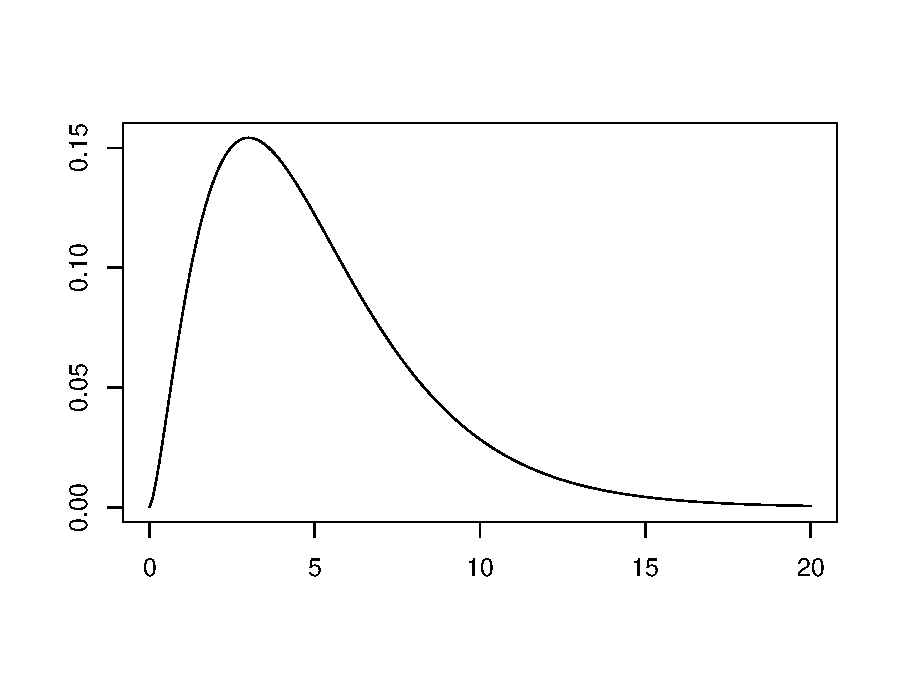
\includegraphics{./dibujos/03/-001}
%\begin{center}
%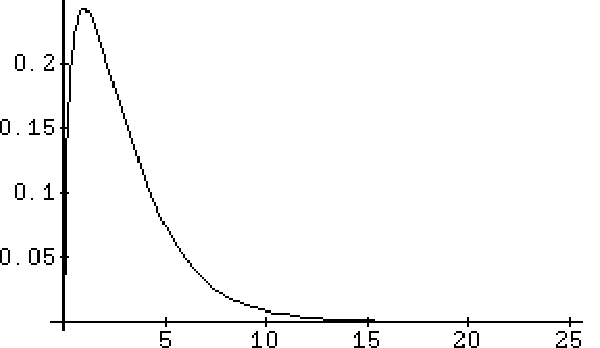
\includegraphics[scale=0.6]{chi2}
%\end{center}
\caption{Gráfica de la función de densidad de la $\chi^2_5$}
\end{figure}


%%\def\dibuixa{\scaledpicture 99.4mm by 61.3mm (c scaled 500)}

%%\dibuixa
\end{frame}

\begin{frame}
%Su función de distribución se puede calcular pero para nuestra comodidad está tabulada.
\frametitle{Ejemplo:}
      El aumento del peso diario de un pollo de una granja sigue una
        distribución normal con desviación típica $1.7$. Se toma una
        muestra de 12 pollos.
        \begin{enumerate}[a)]
            \item Hallar la probabilidad de que la desviación típica muestral
            sea menor que 2.5.
            \item Hallar la probabilidad de que la desviación típica
            muestral sea mayor que 1.
            \end{enumerate}
        
\end{frame}
\begin{frame}
\textbf{Solución}
Sea $X$= el aumento del peso diario de un pollo. Sabemos que $\sigma_{X}^2=(1.7)^2$. Además, como la
distribución de la población es normal y $n=12$, tenemos que
$\frac{(n-1)\tilde{S}_{X}^2}{\sigma_{X}^2}$ sigue  una distribución $\chi^2_{11}$.
\begin{itemize}
\item  $P(\tilde{S}_{X}<2.5)=
P(\tilde{S}_{X}^2<(2.5)^2)=P(\frac{(12-1)\tilde{S}_{X}^2}{(1.7)^2}<\frac{(12-1)
(2.5)^2}{(1.7)^2})= P(\chi_{11}^2<23.7889)\approx P(\chi_{11}^2<24.725)=0.99.$
\item
$P(\tilde{S}_{X}>1)=P(\tilde{S}_{X}^2>1)=P(\frac{(12-1)\tilde{S}_{X}^2}{1.7^2}>\frac{(12-1)
1}{1.7^2})=P(\chi_{11}^2>3.80623)\approx 1-P(\chi_{11}^2<3.816)=1-0.025=0.975$
\end{itemize}
\end{frame}
